\section{Wirtschaft}

\begin{aufgabe}
zu eingebunden -- siehe Hefter
\end{aufgabe}

\begin{itemize}
\item \jar{Rettung} der Bauern -- Ernährungs- und Lebensgrundlage
\item \jar{Rettung} der Arbeiter --
\textquote[{\mycite[139]{DeuzwDemuDikt}}]{umfassende[r] Angriff
gegen die Arbeitslosigkeit}
\item Autarkie $\Rightarrow$ Krieg
\end{itemize}

\begin{figure}
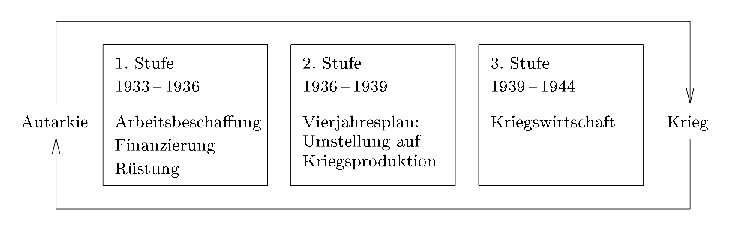
\includegraphics[width=\textwidth]{hit-stufpla.eps}
\caption{\Nam{Hitler, Adolf}{Hitler}s Stufenplan}
\label{pic:hit-stufpla}
\end{figure}

Diese Ziele wollte \Nam{Hitler, Adolf}{Hitler} mit seinem
\ges{Stufenplan} (siehe \ref{pic:hit-stufpla}) erreichen. Dessen erste
Stufe soll hier näher beleuchtet werden. \mar{Und die anderen?}

Die dargestellten Maßnahmen folgten der Politik des \emph{deficit
spending}\index{deficit spending}, welches durch den
Reichswirtschaftsminister und Reichsbankpräsidenten \Nam{Schacht,
Hjalmar}{Hjalmar Schacht} angeregt wurde. Er erfand auch das
sogenannte \emph{Mefo-Wechselsystem}\index{Mefo-Wechsel} zur
Finanzierung der Rüstungsaufträge. Nach diesem bezahlte nicht das
Deutsche Reich direkt selbst, sondern eine Scheinfirma, die \Ins{Mefo,
Metallurgische Forschungsgesellschaft}{Metallurgische
Forschungsgesellschaft} (Mefo) akzeptierte von der Industrie
ausgestellte Wechsel, die bis 1938 einzulösen waren. Die weiteren
Details sind hier unwichtig. Dieses System bot einige
Vorteile.\mar{Doch welche?}


\subsection{Erste Stufe: Wirtschafts- und
Sozialpolitik\mycite{LemoWirtsch}}
\mar{Wo sind die anderen?}

\subsubsection{wirtschaftliche Maßnahmen:}

\begin{itemize}
\item leichter Wirtschaftsaufschung 1933 durch die
Arbeitsbeschaffungsmaßnahmen der vorherigen Regierungen
\item Arbeitsbeschaffungsprogramme (Straßenbau: Autobahn, Bauwesen:
Wohnungsbau) steuerliche Anreize $\Rightarrow$ Senkung der
Arbeitslosigkeit
\item ab \dat{Juni 1935 Reichsarbeits- und Wehrdienst} $\Rightarrow$
Senkung der Arbeitslosigkeit
\item NS-Regime baut auf Privateigentum -- Interessenübereinstimmung
zwischen Großindustrie (Profitgier) und NS-Regime (forcierte
Kriegsvorbereitung)
\item schnelle Aufrüstung der modernen Industriezweige, beispielsweise
des Fahrzeugbaus
\item öffentliche Wirtschaftsforderung, vor allem durch
Rüstungsaufträge
\item Förderung der Landwirtschaft durch das
\dat{\ges{Reichserbhofgesetz} vom 29. September 1933}, das 
Hofteilung, Verkauf und Belastung mit Hypotheken verbot, dadurch aber
auch Neuinvestitionen stark behinderte.
\end{itemize}

\subsubsection{sozialpolitische Maßnahmen:}

\begin{itemize}
\item 1. Mai als staatlicher Feiertag bei voller Lohnfortzahlung
(1933 \ins{Feiertag der nationalen Arbeit}, ab 1934 \ins{Nationaler
Feiertag}) \index{1. Mai}
\item Gründung der Organisation \dat{\ins{Kraft durch Freude} im
November 1933} $\Rightarrow$ kulturelle und touristische
Freizeitbeschäftigungen für große Teile der Arbeiterschaft
\item Sofortmaßnahmen gegen Hunger, Armut und Verelendung, darunter
die Gründung des \dat{\Ins{Winterhilfswerk}{Winterhilfswerks}}
\end{itemize}

\endinput
